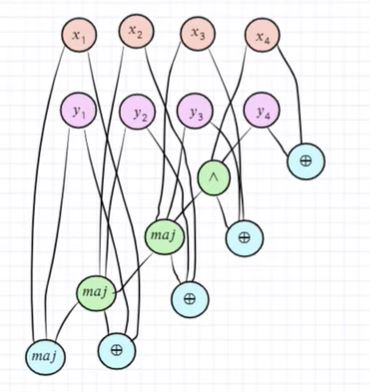
\includegraphics[]{images/26_bad_scheme.JPG}

Это плохая схема, так как чем длиннее цепочка зависимости; чтобы посчитать результат в некотором разряде, нужно посчитать перенос, а для этого результат в предыдущем разряде и.т.д.; поэтому будем делать быстрые сумматоры.

\begin{theorem} Функцию сложения можно вычислить схемой размера $O(n\log n)$ и глубины $O(\log n)$ \end{theorem}

\begin{proof}

Идея состоит в том, чтобы некоторым образом получить биты переноса заранее и потом сложить их с битами чисел параллельно в каждом разряде.

Пусть даны два числа в двоичной записи: $a = \overline{a_1 \ldots a_n}$ и $b = \overline{b_1 \ldots b_n}$. Для простоты будем считать, что $n$ ~--- степень двойки. Цель состоит в том, чтобы для каждого разряда найти бит переноса $c_i$, чтобы затем получить в каждом разряде результат $s_i = a_i \oplus b_i \oplus c_i$ (таким образом, $c_i = 1$, если есть перенос из $(i+1)$-го разряда в $i$-й, при этом нумерация начинается с нуля, поскольку в сумме на один разряд больше). Но в процессе нужно найти промежуточные биты генерации и проталкивания. Введем определения:

\begin{itemize}
    \item $g_{i\ldots j} = 1$ (блок $i\ldots j$ генерирует перенос), если при сложении $\overline{a_i \ldots a_j}$ и $\overline{b_i \ldots b_j}$ образуется перенос 
    \item $p_{i\ldots j} = 1$ (блок $i\ldots j$ проталкивает перенос), если при сложении $\overline{a_i \ldots a_j}$ и $\overline{b_i \ldots b_j}$ образуется число из одних единиц: блок сам по себе не образует переноса, но если придет перенос из младших разрядов, то он "протолкнется" в более старшие.
\end{itemize}

Далее мы последовательно вычислим биты генерации и переноса для всех "выровненных" блоков с длинами ~--- степенями двойки.

Заметим, что 

\begin{itemize}
    \item $g_{i\ldots i} = a_i \wedge b_i$ (перенос появляется, если оба слагаемых единицы)
    \item $p_{i\ldots i} = a_i \oplus b_i$ (по определению)
    \item $\forall k: i \le k \le j \; g_{i\ldots j} = g_{i\ldots k} \vee (g_{k+1\ldots j} \wedge p_{i\ldots k})$
    \item $\forall k: i \le k \le j \; p_{i\ldots j} = p_{i\ldots k} \wedge p_{k+1\ldots j}$
\end{itemize}

Тогда, за базу возьмем блок из одного бита. Далее переход осуществляем следующим образом: разбиваем блок $i\ldots j$ на два подблока $i\ldots k$ и $k+1 \ldots j$ и считаем для него биты генерации и проталкивания как описано выше. 
Поскольку каждый блок добавляет константу новых элементов, а всего рассматривается $O(n)$ блоков, общий размер построенной схемы равен также $O(n)$. Глубина же будет логарифмической, поскольку каждый блок использует результаты двух блоков вдвое короче. 

Теперь посчитаем биты переноса. Для каждой позиции $i$ разобьем весь хвост $i \ldots n$ на блоки, для которых посчитаны биты генерации и переноса. Если действовать жадным алгоритмом, начиная с конца, то для каждой длины будет взято не больше одного блока, поэтому общее число блоков не привысит $\log n$. Обозначим эти блоки цифрами $1, \ldots, q$. Тогда бит переноса можно найти по формуле $$c_i = g_1 \vee (g_2 \wedge p_1) \vee (g_3 \wedge p_2 \wedge p_1) \vee \ldots \vee (g_q \wedge p_{q-1} \wedge \ldots \wedge p_1)$$
Действительно, перенос либо возник в первом блоке, либо возник во втором и протолкнулся через первый, либо возник в третьем и
протолкнулся через первые два, и так далее. Поскольку $q = O(\log n)$, размер схемы для вычисления одного бита переноса будет также $O(\log n)$, а для вычисления всех битов переноса $O(n\log n)$. Глубина же добавится константная (если разрешить только элементы с двумя входами, то повторный логарифм).

Таким образом, схема состоит из трёх этапов: вычисление битов генерации и проталкивания для блоков, затем вычисление битов переноса для разрядов и, наконец, вычисление результатов. Общий размер составляет $O(n\log n)$, а глубина ~--- $O(\log n)$, как и было заявлено. Таким образом, сложение лежит в $\nc^1$ \end{proof}